\chapter{Complementary-Filter}
\label{chap:ComplementaryFilter}

The first approach for a sensor fusion is the complementary filter. This filter uses a highpass filter for the gyroscopes and a lowpass filter for the acceleration sensor. The highpass filter is used after the integration of the rotation rates. This can be seen in figure \ref{fig:complementary}.\\
\begin{figure}[H]
	\centering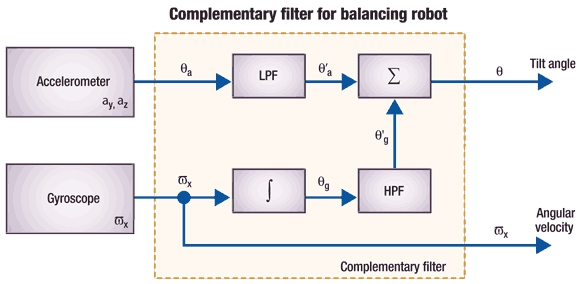
\includegraphics[width=1\textwidth]{fig/Complementary.jpg}
	\caption{Complementary-Filter\cite{doc:STM}}
	\label{fig:complementary}
\end{figure}
The implementation effort is extremely lower than with the Kalman Filter. Because here not matrices and matrix operations are needed. Also are there less calculations and so fits this algorithm better to microprocessors. The only thing what needs to be checked is the lowpass/highpass-filter coefficient. Next the needed calculations are mentioned to show the difference of the complementary and Kalman filter.
\begin{itemize}
	\item Calculation of the accelerometer and magnetometer angles
	\item Calculation of the gyroscope angles
	\item Complementary-Filter usage with defined filter time of the lowpass and highpass-filter
\end{itemize}